\documentclass[twocolumn]{article}

\usepackage{graphicx}   
\usepackage{url}        
\usepackage{amssymb}
\usepackage{amsmath}    
\usepackage{booktabs} 
\usepackage{amsmath}
\usepackage{subfigure}
% \usepackage{hyperref}


\usepackage[colorlinks,citecolor=blue,linkcolor=blue,bookmarks=false,hypertexnames=true, urlcolor=blue]{hyperref} 
% \renewcommand{\@biblabel}[1]{#1.} % Заменяем библиографию с квадратных скобок на точку:

\renewcommand{\theenumi}{\arabic{enumi}}% Меняем везде перечисления на цифра.цифра
\renewcommand{\labelenumi}{\arabic{enumi}}% Меняем везде перечисления на цифра.цифра
\renewcommand{\theenumii}{.\arabic{enumii}}% Меняем везде перечисления на цифра.цифра
\renewcommand{\labelenumii}{\arabic{enumi}.\arabic{enumii}.}% Меняем везде перечисления на цифра.цифра
\renewcommand{\theenumiii}{.\arabic{enumiii}}% Меняем везде перечисления на цифра.цифра
\renewcommand{\labelenumiii}{\arabic{enumi}.\arabic{enumii}.\arabic{enumiii}.}% Меняем везде перечисления на цифра.цифра



% Some useful/example abbreviations for writing math
\newcommand{\argmax}{\operatornamewithlimits{argmax}}
\newcommand{\argmin}{\operatornamewithlimits{argmin}}
\newcommand{\x}{\mathbf{x}}
\newcommand{\y}{\mathbf{y}}
\newcommand{\ypred}{\mathbf{\hat y}}
\newcommand{\yp}{{\hat y}}

\begin{document}

% Define document title, do NOT write author names for the initial submission
\title{INF-584 project: LightCuts}
\author{Amelichev Konstantin}
\maketitle

% Write abstract here
\begin{abstract}
    During project I researched LightCuts technique and it's different approaches.
    I wrote an implementation of LightCuts based on CPU raytracer in MyRenderer, assignment codebase for INF-584.
    Source code can be found at \href{https://github.com/KiK0S/my-lightcuts}{Github}.
\end{abstract}

% Each section begins with a \section{title} command
\section{Introduction}
\label{sec:intro}
\subsection{Ray Tracing}

Ray tracing is a rendering technique that simulates the behavior of light rays to generate realistic images. In ray tracing, a ray is cast from the camera through each pixel in the screen space. The intersection of this ray with scene geometry determines the color of the corresponding pixel in the image. This process involves evaluating lighting contributions, considering surface properties, and accounting for shadows.
Ray tracing is computationally expensive, especially for scenes with complex geometry and lighting.
In MyRenderer, BVH structure is used to accelerate intersecion test.

\subsection{Light Models}
Lighting models describe how light interacts with surfaces in a scene, influencing the appearance of objects.

\subsubsection{Phong Model}
The Phong reflection model is a popular empirical lighting model used in computer graphics. It calculates ambient, diffuse, and specular reflection.
However, it may not accurately capture complex lighting interactions, especially in scenes with highly reflective or rough surfaces.


\subsubsection{BRDF (Bidirectional Reflectance Distribution Function)}
The Bidirectional Reflectance Distribution Function (BRDF) is a fundamental concept in computer graphics that describes how light is reflected at a surface point.
It characterizes the relationship between incoming light direction, outgoing light direction, and surface properties such as reflectivity and roughness.

For rendering purposes,
$$L(\omega_o) = \sum L_i(\omega_i) \cdot brdf(\omega_o,\omega_i) \cdot \cos(\omega_i, n)$$

\subsubsection{Cook-Torrance Model}
The Cook-Torrance model is a physically-based lighting model that provides more accurate and realistic results compared to the Phong model.
It is based on microfacet theory, which describes surfaces as composed of numerous microfacets that interact with incoming light rays.

The Cook-Torrance model is highly customizable and allows specifying a lot of different components of the illumination.
As a basic example, diffuse and specular can be used.

\subsubsection{Many lights problem}

For many scenes, light setup is static and some computations can be precalculated before rendering each frame.
At the same time, BRDF approximation of a light emission ideally should account for all the lights, except those not visible from the point.
This is computationally heavy for scenes with a big number of light sources.

\subsubsection{Virtual lights}

Not only number of lights in the scene can be high, but also additional light sources can be added.
For example, it is convinient to approximate area light with a grid of point lights.
And for solving indirect lightning problem, virtual light sources are created near mesh vertices.
For instance, in Point-based globall illumination algorithm, surflets are created from mesh point cloud, and each surflet is a light source.

\section{Overview of lightCuts}

LightCuts is a technique used to accelerate the rendering process in scenes with many light sources.
It efficiently approximates the illumination of a scene by selecting a subset of lights that contribute the most to the final image.
By reducing the number of lights considered during rendering, LightCuts significantly improves rendering performance without sacrificing visual quality.

To select contributors to light at specific point, a light tree is used.
It stores all the light sources in a scene, and each node represents an unbiased estimator of underlying set of lights.
Each node has an error bound calculated, being a maximal potential contribution to illumination.
Then lightcuts takes more representatives from nodes that contribute the most to illumination, eventually selecting a subset of tree nodes.

\subsection{Building Light Tree}

Light tree is built in an bottom-to-top way, having initially $n$ light sources as $n$ nodes, and merging nodes with high proximity together.
Each node stores a pointer to two children, bounding box of subtree's lights, total intensity of subtree's lights, and a single light representative.
For selecting clusters to merge, original paper uses score $I \cdot (a^2 + b \cdot (1 - \cos c))$, where $b$ is 0 for point and directional lights.
As in this project LightCuts is only studied for point lights I will further go with $I \cdot a^2$, where $I$ is a total intensity of lights and $a$ is a squared diagonal of cluster's bounding box.

The basic building operation takes $O(n^3)$ time, which is computationally heavy, but it is a single run before rendering all the frames.
It can also be improved if not every cluster pair is scored (based on some order, preserving locality) and if caching is introduced.

\subsection{Selecting Light Cut}
Once the light tree is constructed, each LightCuts query aims to receive a set of lights that approximates the scene.
To do that, top-to-bottom approach is used: we estimate illumination by root node, and then refine the estimate based on error upper bound.

For instance, if we know that root's bounding box is far away from the requested position, than we can use light source estimator from the root node.
Otherwise, we split node in two, refine our estimators and repeat the process.

Typically, 2\% threshold is used --- if node is responsible for less than 2\% of total illumination, it can be approximated by a random cluster representative.

\subsection{Calculation of an Error Upper Bound}

Error upper bound is stored in tree nodes to provide information on maximal potential influence of current node on illumination.
For that, we calculate an upper bound value of node contribution to illumination.
For instance, for point lights, we imagine that all light sources are in the closest corner of bounding box, if query point is outside of it.
At the same time for caclulating cosine between normal and light source, we imagine worst scenario as well. 
As a result, we get a number that shows potential contribution of the node to overall illumination.

To bound error, lightcuts bounds all the parts of the illumination equation:

Visibility term is bounded by one, because it is difficult to instantly tell if light is visible or not.

Geometry term for directional lights is bounded by one, and for point lights is bounded by $\frac{1}{d^2}$, where $d$ is a distance between point and bounding box.
Note that for points inside of bounding box we consider error bound as infinite.

For material term, BRDF in use is studied to determine, how it could be affected by lights from a constrained area.
For diffuse part, it is constant, for specular Phong specular was used. It can be extended to other light models as well.
In most cases, to bound BRDF value, cosine needs to be bound as well as constants.

For MyRenderer, following formula based on Phong model was used:

$$ k_d \cdot \frac{1}{\pi} \cdot \cos^*(\omega_i, n) + k_s \cdot \cos^*(2 \cdot \cos(\omega_o, n) \cdot n - \omega_o, w_i)$$

Note that evaluating cosine with light direction involves evaluating upper bound on this cosine.

\section{Implementation}

Implementation was based on MyRenderer code base for INF-584 course assignments.
MyRenderer has a CPU RayTracer, rasterizer with Cook-Terrance lighting model support, BVH for ray tracing speedup. 

For reference implementations, I've looked for open source repositories, but haven't found one, that was focused on lightcuts only and didn't contain bugs at the same time.
Overall, I was referencing a set of implementations, but had to do most of things from scratch, which was time consuming.

\subsection{Choices and Details}

For LightCuts queries I came up with an interface that takes a ray hit description and returns a list of light sources to apply at this pixel.
It was a good decision, becase I always had to compare results with pure evaluation method that takes all lights into account.
As one might notice, the difference between these two methods is just a source of list (either LightCuts instance or scene lights list).

The drawback of this method is the fact that my lightcuts implementation evaluates illumination twice: once for approximation and second time for resulting image.
It can be changed but it won't be as practical during development and research.
Also, it allows estimating error on lightning model not matching one used for rendering.
For example, for basic Phong estimator, Cook-Terrance can be used in scene, if error threshold is low enough.

It should be noted that proper choice of data structure for light cuts was important.
At the start, I used STL set as a heap, because of it's convinience.
As I found later, it reduced performance 2-3 times compared to an STL algorithm for constructing heap on the vector.

There are also several choices related to lightcuts itself, because the original paper is great at providing a short description of a general idea, but details are too vague.
For instance, there is a choice of which light from cluster to return.
One option is to return reference light that was sampled based on intensities, with intensity mapped to cluster intensity.
This option is the one authors use for unbiased estimator.
However, it looses control over what will be displayed: one light might become much more intensive than it was originally.
Another option is to only select one light sample from the node and don't scale its intensity.
It doesn't provide an unbiased estimator, but it's output is predictable, and one can think of it as "selecting only sample of light sources".

After some experiments, I went with the first option, because it was more suitable for homogenious lights that can be grouped.

Another question is whether or not take a different representative light on each frame.
Pros are we can get a better average estimate over region, cons are image will be noisy.
This is a base of a separate research paper "Stochastic lightcuts", because sampling should have probability functions relevant to lights geometric properties.
Authors noted that wrong sampling strategy shouldn't be any better than intensity-based sampling strategy, so I went for the intensity based one as most primitive.
Overall, I have both strategies available, sample or take static representative.
Sampling, indeed, leads to some noise in final image.

To speed up error calculation, I used timer variable, that is updated for every new ray.
Each node stores it's own timer and cached error upper bound.
With timer I can check in $O(1)$ if node needs to recalculate error.
The same mechanism is applied for light evaluation.

\section{Evaluation and Results}

LightCuts is not the most cpu-friendly algorithm for testing, because it has a base complexity of $O(n^3)$ for building,
which gives an upper bound for number of lights for testing around 1000, after that it will be too slow.
At the same time, it has an overhead compared to naive approach, which should be neglected at large scale, but is noticable for small number of lights.
Not only that, but approximation error gets unnoticable at around 1000 lights point mark, so effectively testing lightcuts is a problem.

I am using a proxy-metric, such as average number of lights evaluted for each ray. For naive approach it will be always the number of lights in the scene.

For the test setups, I modified MyRenderer so it has several ray tracers and pressing TAB just changes current view. It is much better for Ray tracers comparison.
There are 5 total setups: Rasterizer with Cook-Terrance model, RayTracer, RayTracer + LightCuts, RayTracer + LightCuts + sampling, RayTracer + LightCuts but without strong specular estimate.
All ray tracer environments have a second preview mode that generates small version of an image.

For scenes, I've modelled a basic scene of a table with a monitor on it. This monitor acts like an area light. I procedurally put a lot of pixels on it, that emit light as a point source.
There are two demos for that - one with blank screen, that verifies grouping point lights together.
Another demo has a white background and a red line on a screen. It checks if LightCuts loses some information while grouping lights.

Another scene I used was an open model of a low poly bedroom. For this scene, I sampled a cloud of point lights.


\subsection{results}

For area light, there were a minor difference in quality between pictures. At the same time, performance for lightcuts was much worse. Because of the scene structure, not only it had to build a tree but also to check most of the lights.

For scattered lights, LightCuts was noticably faster event for modest scene with 100 lights. however, when it groups lights of different structure, it creates a lot of noise.
One way to take care of that was to set a high error bound on specular light, so only diffuse part really makes difference;
Another way was using hierarchical sampling. It created some noise but overall it recovered structure much better.
If it wasn't so computationally heavy, there also could be an experiment with sampling several lights and taking an average while taking a cut and approximating a light.

Images and benchmarks are given in the report, but it is strongly advised to check them at github page in case final set of experiments wasn't finished before deadline. https://github.com/KiK0S/my-lightcuts 




\begin{table}[h]
    \centering
    \begin{tabular}{|p{1cm}|p{2.5cm}|p{1.5cm}|p{1.5cm}|}
    \hline
    Demo Name & Configuration & Time to Render (ms) & Lights Evaluated (Avg) \\ \hline
    desk \[\ref{fig:desk}\] & Ray tracer & 146,412 & 216  \\ \hline
    desk \[\ref{fig:desk}\]  & Ray tracer + LightCuts & 416,560 & 107.464 \\ \hline
    desk \[\ref{fig:desk}\]& Ray tracer + LightCuts, no specular estimate & 490,178 & 126.222  \\ \hline
    desk \[\ref{fig:desk}\]& Ray tracer + LightCuts + sampling & 462,235 & 107.735 \\ \hline
    \end{tabular}
\end{table}


\begin{table}[h]
    \centering
    \begin{tabular}{|p{1cm}|p{2.5cm}|p{1.5cm}|p{1.5cm}|}
    \hline
    Demo Name & Configuration & Time to Render (ms) & Lights Evaluated (Avg) \\ \hline
    desk-red \[\ref{fig:desk-red}\] & Ray tracer & 93,203 & 216  \\ \hline
    desk-red \[\ref{fig:desk-red}\] & Ray tracer + LightCuts & 415,544 & 159.074 \\ \hline
    desk-red \[\ref{fig:desk-red}\] & Ray tracer + LightCuts + sampling & 393,013 & 132.27 \\ \hline
    \end{tabular}
\end{table}



\begin{table}[h]
    \centering
    \begin{tabular}{|p{1cm}|p{2.5cm}|p{1.5cm}|p{1.5cm}|}
    \hline
    Demo Name & Configuration & Time to Render (ms) & Lights Evaluated (Avg) \\ \hline
    bedroom \[\ref{fig:bedroom}\] & Ray tracer & 75,527 & 100  \\ \hline
    bedroom \[\ref{fig:bedroom}\] & Ray tracer + LightCuts & 80,019 & 75.1403 \\ \hline
    bedroom \[\ref{fig:bedroom}\]& Ray tracer + LightCuts, no specular estimate & 100,974 &89.6361 \\ \hline
    bedroom \[\ref{fig:bedroom}\] & Ray tracer + LightCuts + sampling &   90,079&    72.5656\\ \hline
    \end{tabular}
\end{table}


\section{Conclusions}

Overall, LightCuts is a tricky algorithm.
It's basis is trivial and is associated with yet one more hierarchical structure for speeding ray tracing.
However, it is much harder than, for instance, BVH, because of how minor errors dont lead to inefficient result, but to a result that seems correct even though is far from truth.

During this project implementation of lightcuts was created for Phong lighting model and several heuristics were adopted.



\paragraph{References} \hfill

Fernandez, B. W. S., Arbree, A., Bala, K., Donikian, M., \& Greenberg, D. P. Lightcuts: A Scalable Approach to Illumination., \href{https://www.cs.cornell.edu/~kb/projects/lightcuts/lightcuts.pdf}{URL}


Yuksel, C. (2019, July). Stochastic lightcuts. In Proceedings of the Conference on High-Performance Graphics (pp. 27-32)., \href{http://www.cemyuksel.com/research/stochasticlightcuts/stochasticlightcuts.pdf}{URL}


Mikšık, M. Implementing Lightcuts., \href{https://citeseerx.ist.psu.edu/document?repid=rep1&amp;type=pdf&amp;doi=36fc192f1d104453dce63644e9723332ae08bb4c}{URL}


Christensen, P. H. (2010, July). Point-based global illumination for movie production. In ACM SIGGRAPH (Vol. 1). \href{https://graphics.pixar.com/library/PointBasedGlobalIlluminationForMovieProduction/paper.pdf}{URL}

Abhinav Gupta, Ranveer Aggarwal. lightcuts-pbrt, \href{https://github.com/ranveeraggarwal/lightcuts-pbrt}{Github}


Bus, N., Mustafa, N. H., \& Biri, V. (2015, May). IlluminationCut. In Computer Graphics Forum (Vol. 34, No. 2, pp. 561-573), \href{https://github.com/winmad/IlluminationCut}{Github}




\begin{figure}[htbp]
    \centering
    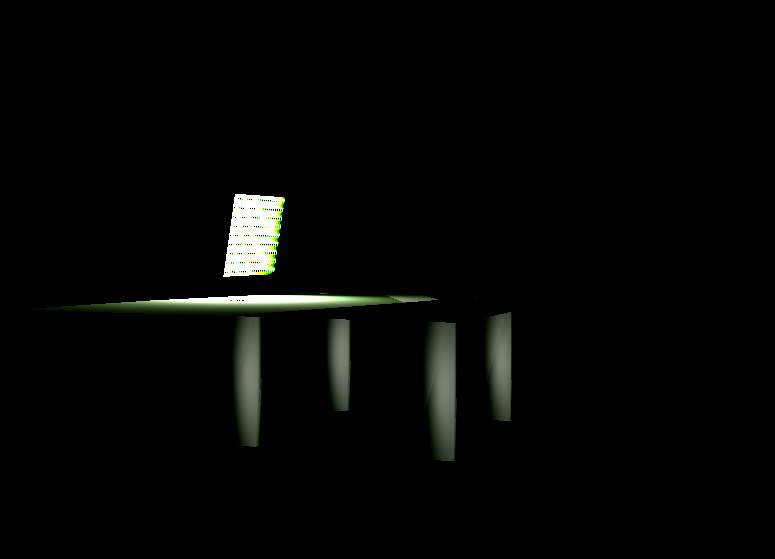
\includegraphics[height=5cm]{img/desk-1.png}
    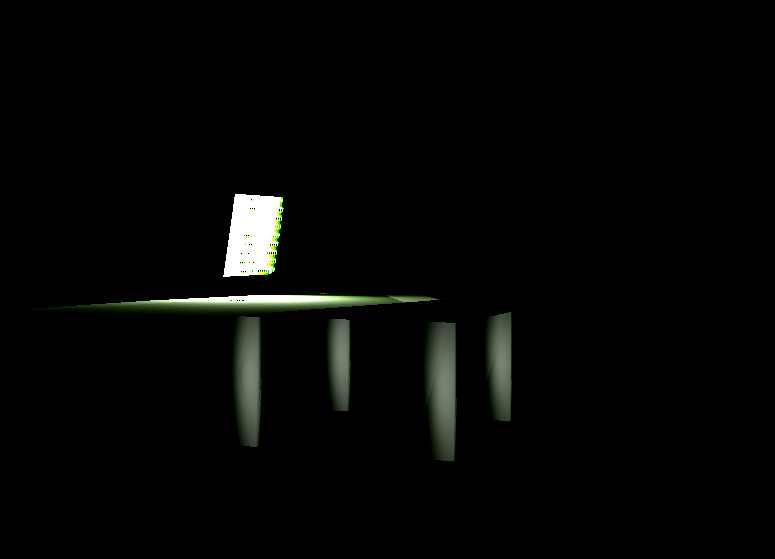
\includegraphics[height=5cm]{img/desk-2.png}
    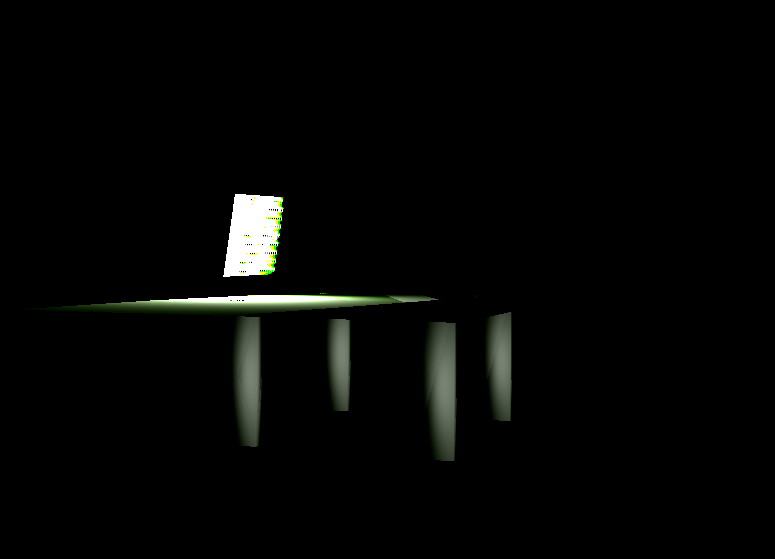
\includegraphics[height=5cm]{img/desk-3.png}
    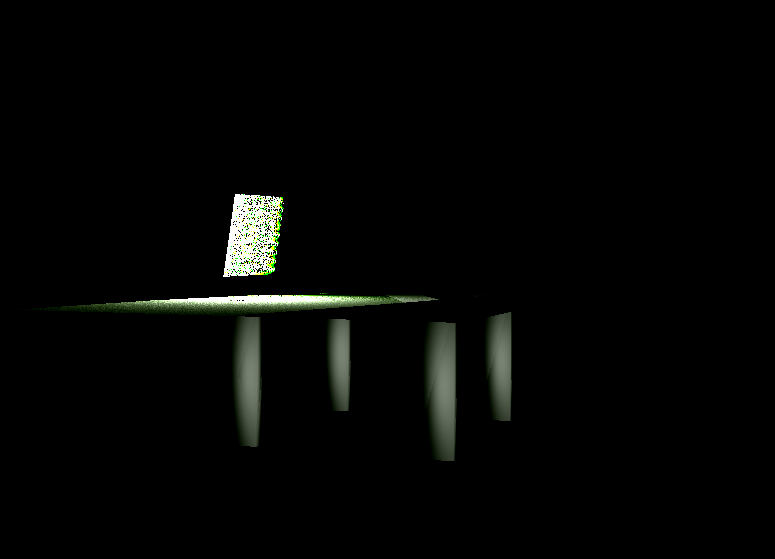
\includegraphics[height=5cm]{img/desk-4.png}
    \caption{Desk experiment}
    \label{fig:desk}
\end{figure}


\begin{figure}[htbp]
    \centering
    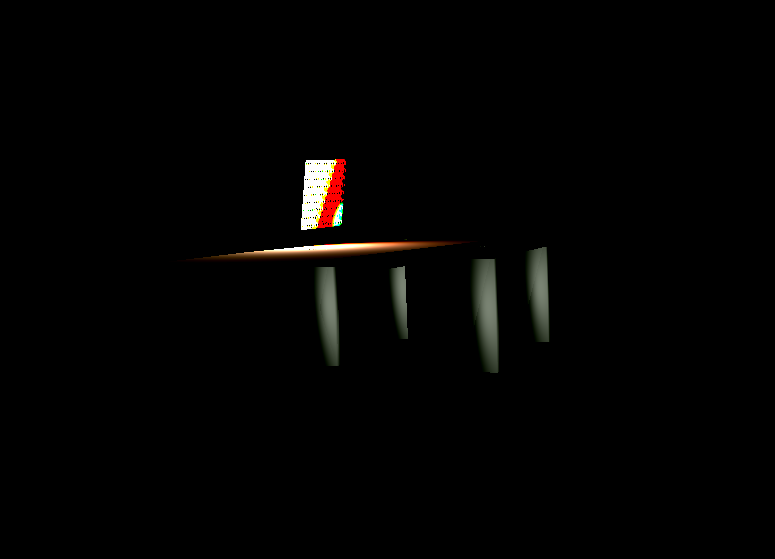
\includegraphics[height=5cm]{img/desk-red-1.png}
    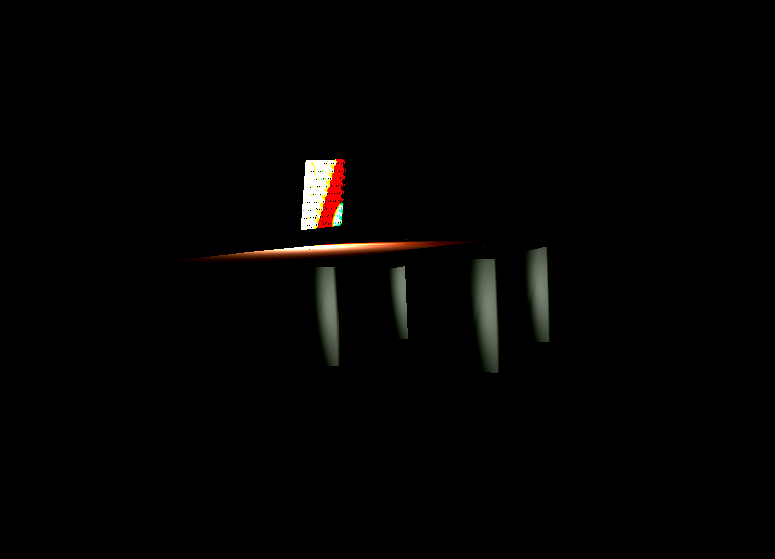
\includegraphics[height=5cm]{img/desk-red-2.png}
    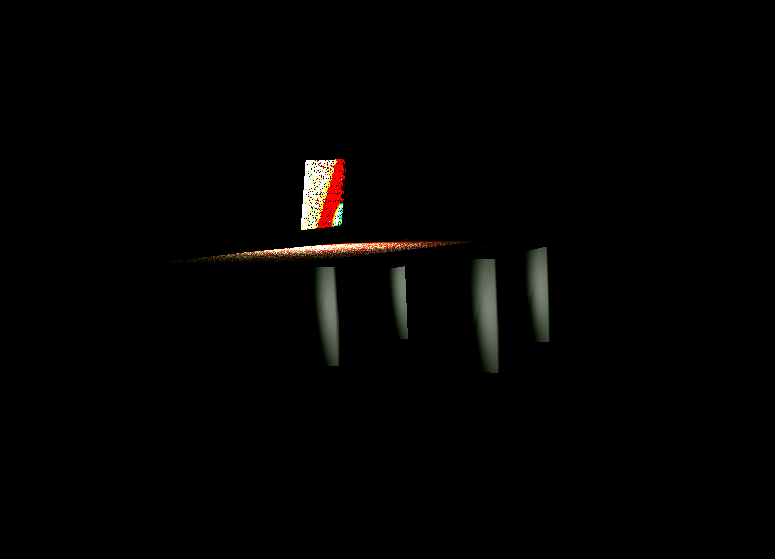
\includegraphics[height=5cm]{img/desk-red-3.png}
    \caption{Desk experiment with red line}
    \label{fig:desk-red}
\end{figure}



\begin{figure}[htbp]
    \centering
    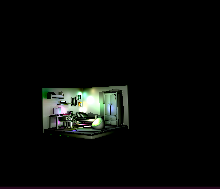
\includegraphics[height=5cm]{img/bedroom-1.png}
    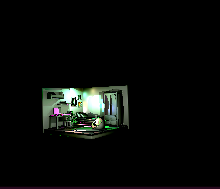
\includegraphics[height=5cm]{img/bedroom-2.png}
    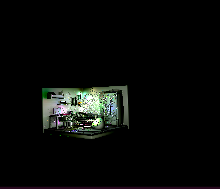
\includegraphics[height=5cm]{img/bedroom-3.png}
    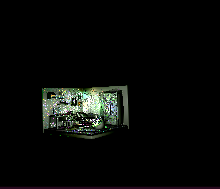
\includegraphics[height=5cm]{img/bedroom-4.png}
    \caption{Bedroom scene}
    \label{fig:bedroom}
\end{figure}

\end{document}
